% Appendix A

\chapter{CR3 Register Introduction} % Main appendix title

\label{AppendixA} % For referencing this appendix elsewhere, use \ref{AppendixA}

\lhead{Appendix A. \emph{CR3 Register Introduction}} % This is for the header on each page - perhaps a shortened title

The CR3 register is a typical hardware anchor [3] where we could derive some OS-level information in the context of derivative 
pattern VMI. Since our study is about how to leverage derivative pattern in monitoring network traffic on per-process basis, it’s 
better to resume the CR3’s functionality and explore its potentiality for future usage. This is the motivation of this work and the 
remainder of this article is organized as follow. In the first part, some background conceptions about memory addressing, involved 
in the functioning of CR3 register, will be presented. Subsequently, we talk about how CR3’s functionality specified in Intel 
developer manual [2] and helps in translating a linear address into a physical address. In the end, we address how CR3 register 
is leveraged to derive or infer system process information and its potentiality in network traffic monitoring. 

\section{Background \cite{BookLinuxKernel}}
To well understand the functionality of CR3 register, some basic and related conceptions about memory addressing should be kept in
mind.

\begin{itemize}
 \item\textbf{Logical Address}: consists of a segment and an offset, included in the machine language instructions to specify the address of an 
operand or an instruction.
 \item\textbf{Linear Address}: also known as virtual address, a single 32 bits unsigned integer that can be used to address up to 4GB. Their values
range from 0x00000000 to 0xffffffff.
 \item\textbf{Physical Address}: used to address memory cell in memory chips.
 \item\textbf{MMU}: Memory Management Unit, a hardware circuit integrated in x86 architecture and it consist of two parts:  
Segmentation Unit helping CPU translate a logical address into a linear address and Paging Unit capable of transforming a linear
address into a physical address.
\end{itemize}

\begin{figure}[htbp]
	\centering
		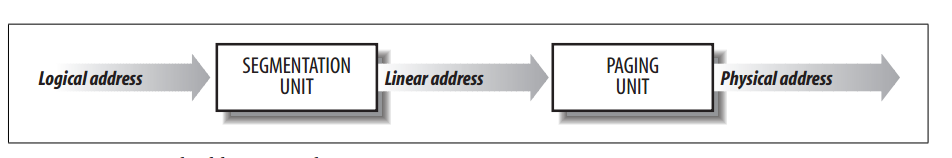
\includegraphics[width=13cm, height= 4cm ]{Figures/FigureAppendix1.png}
	\caption{Logical Address Translation \cite{BookLinuxKernel}}
	\label{fig:Logical Address Translation}
\end{figure}

Segmentation has been included in 80x86 microprocessors to encourage programmers to split their applications into logically related
entities, such as subroutines or global and local data areas. However, Linux uses segmentation in a very limited way. In fact, 
segmentation and paging are somewhat redundant, because both can be used to separate the physical address spaces of processes: 
segmentation can assign a different linear address space to each process, while paging can map the same linear address space into 
different physical address spaces. Linux prefers paging to segmentation.

\section{Functionality of CR3 Register \cite{BookIntelManuel}}
CR3 register is a control register integrated in CPU. Along with other control registers such as CR0, CR1, CR2, CR3 and CR4, they 
are used to determine operating mode of the processor and the characteristics of the currently executing task. This section presents
control register in the perspective of processors.

\begin{figure}[htbp]
	\centering
		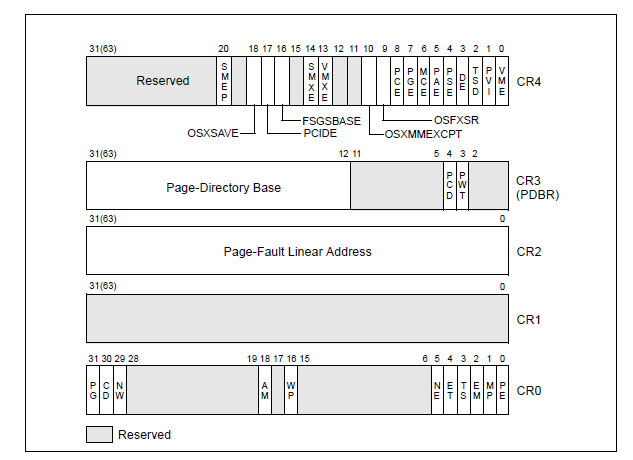
\includegraphics[width=13cm, height= 8cm ]{Figures/FigureAppendix2.png}
	\caption{Control Register Architecture \cite{BookIntelManuel}}
	\label{fig:Control Register Architecture}
\end{figure}

Figure \ref{fig:Control Register Architecture} presents the four control registers’ architecture. Their respective functionalities are
summarized below, and each architecturally defined control field in these control registers are described individually.

\begin{itemize}
 \item\textbf{CR0}: contains system control flags that control operating mode and states of the processor.
 \item\textbf{CR1}: reserved.
 \item\textbf{CR2}: contains the page-fault linear address (the linear address that caused a page fault).
 \item\textbf{CR3}: contains the physical address of the base of the paging-structure hierarchy and two flags (PCD and PWT). Only the
 most-significant bits (less the lower 12 bits) of the base address are specified; the lower 12 bits of the address are assumed to be
 0. The first paging structure must thus be aligned to a page (4-KByte) boundary. The PCD and PWT flags control caching of that paging
 structure in the processor’s internal data caches (they do not control TLB caching of page-directory information). CR3 register works
 on condition that VIRTUAL ADDRESSING feature is enabled, which means that PG bit is set in CR0.
 \item\textbf{PCD}: Page-level Cache Disable (bit 4 of CR3) — Controls the memory type used to access the first paging structure of 
 the current paging-structure hierarchy. This bit is not used if paging is disabled, with PAE paging, or with IA-32e paging if CR4.
 PCIDE=1. Please refer to Section 4.9: “Paging and Memory Typing” in reference [] to get more information.
 \item\textbf{PWT}: Page-level Write-Through (bit 3 of CR3) — Controls the memory type used to access 
\end{itemize}

\section{Functioning of CR3 Register in Memory Addressing}
Figure \ref{fig:Paging by 80x86 Processors} well explains how MMU uses CR3 register to translate a linear address into a physical one.
The 32 bits linear address can be divided into 3 parts: Directory (the most significant 10 bits), Table (the intermediate 10 bits) and
Offset (the least significant 12 bits). The physical address of the Page Directory in use is stored in a control register named CR3. 
The Directory field within the linear address determines the entry in the Page Directory that points to the proper Page Table. The 
address’s Table field, in turn, determines the entry in the Page Table that contains the physical address of the page frame containing
the page. The offset field determines the relative position within the page frame.

\begin{figure}[htbp]
	\centering
		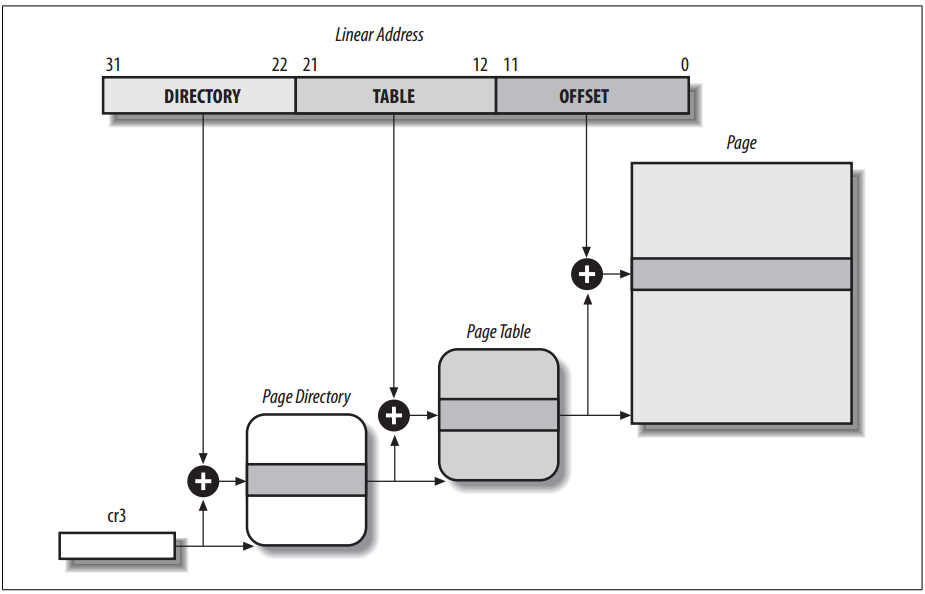
\includegraphics[width=13cm, height= 8cm ]{Figures/FigureAppendix3.png}
	\caption{Paging by 80x86 Processors}
	\label{fig:Paging by 80x86 Processors}
\end{figure}

Since the CR3 register holds the address of the top-level Page Directory for the current context and a single address space is active
per processor at any given time, the physical address stored in CR3 register could be used to represent its unique corresponding 
process. This is the theoretical base for that CR3 could be profited in the derivative pattern. For example, a new CR3 value means 
a new process has been created, a transition from one to another value in CR3 means that a context switch (process switch) has 
occurred. Antfarm \cite{Reference4} has leveraged this characteristic to enumerate all executing processes, monitor the creation, switch and exit of 
process. However, in Antfarm, cause of the limitation of derivative pattern, we could just get its page directory base address and 
executing time for each identified process. Due to the lack of semantic knowledge for kernel memory, it is impossible to get more 
detailed information (such as PID, process name, etc.) about identified processes. Based on Antfarm, Lycosid \cite{Reference9} whose 
objective is to detect the hidden malicious processes has been developed. Its idea is to compare a process list deduced by low-level 
hardware with that obtained by some system utility such as UNIX command “ps”. In case of inconsistency about process number, Lycosid
infers the presence of hidden processes in monitored VM and identify those processes in a statistical manner.













